%There are two parts.
%\begin{itemize}
%\item Estimate
%\item Exact
%\end{itemize}
Let the frequency offset be 
$\Delta f$  
\cite{freq_offset}
.  Then
\begin{align}
\label{eq:freq_offset_model}
\vec{y}_k= \vec{x}_k e^{j2\pi\Delta fkT_s} + \vec{n}_k, \quad k = 1,\dots,N 
\end{align}  
where $T_s \le \frac{1}{2\Delta f}$ is the sampling time.

\begin{equation}
\label{eq:freq_offset_model}
Y_k= X_k e^{j2\pi\Delta fkM} + V_k, \quad k = 1,\dots,N 
\end{equation}  
From \eqref{eq:freq_offset_model},
%
\begin{align}
Y_kX_k^*&= \abs{X_k}^2e^{j2\pi\Delta fkM}+ X_k^*{V}_k\\
\implies r_k&=e^{j2\pi\Delta fkM}+ \bar{V}_k
\end{align}
where
\begin{align}
r_k=Y_kX_k^*, \bar{V}_k=X_k^*{V}_k, \abs{X_k}^2=1
\end{align}
%
The autocorrelation can be calculated as
\begin{equation}
R(k) \overset{\Delta}{=} \frac{1}{N-k}\sum_{i=k+1}^{N} r_{i}r^{*}_{i-k}
 , 1 \leq k \leq N-1
\end{equation}
Where N is the length of the received signal.
%DVB-S2 operating with large frequency. So Large frequency offset model has to be employed which is the  Exact approximation of LR technique \cite{1}
For large centre frequency, the following yields a good approximation for frequency offset upto 40 
MHz.
\begin{equation}
\Delta\hat{f} \approx \frac{1}{2\pi M}\frac{\sum_{k=1}^{P}\text{Im}(R(k))}{\sum_{k=1}^{P}k\text{Re}(R(k))},
\quad  P\Delta{f}M << 1
\label{eq:Z}
\end{equation}
%
where $P$ is the number of pilot symbols.
\subsection{Plots}
%\begin{figure}
%\begin{center}
%\includegraphics[width=\columnwidth]{./figs/frequency_best.eps}
%\end{center}
%\caption{Error variation with respect to frequency offset.  }
%\label{fig:freq_best}
%\end{figure}
%%
%\begin{figure}
%\begin{center}
%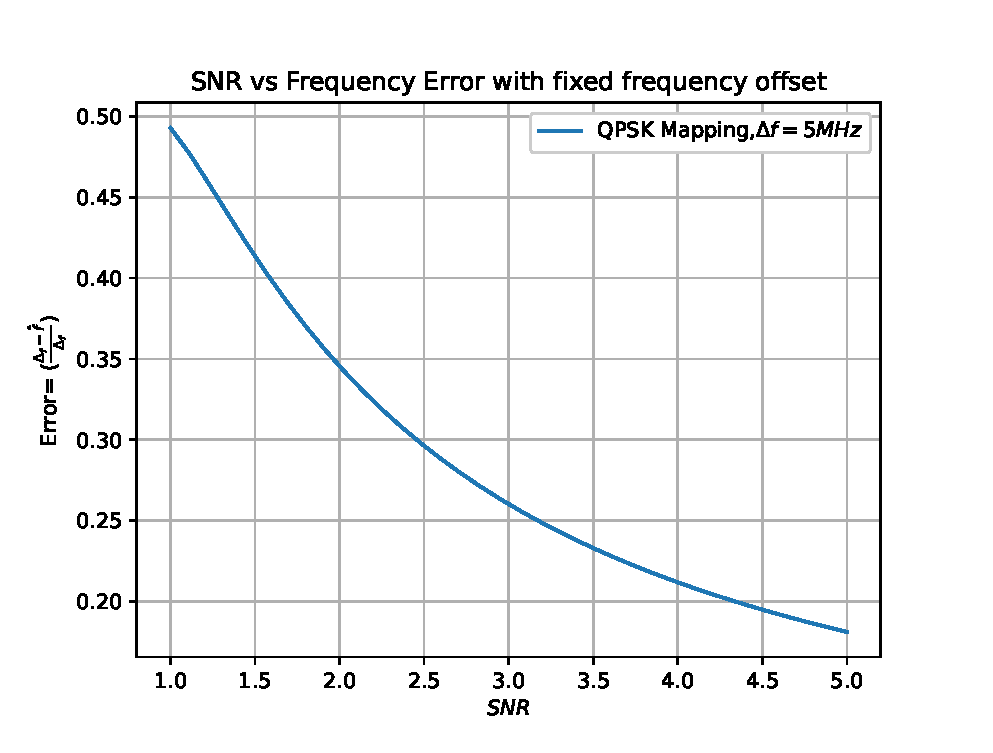
\includegraphics[width=\columnwidth]{./figs/frequencyestiamtion_best_error_vs_snr.eps}
%\end{center}
%\caption{Error variation with respect to the SNR.  $\Delta f = 5$ MHz, Center frequency $f_c=25$ GHz}
%\label{fig:freq_est}
%\end{figure}

%
The number of pilot symbols is $P = 18$. The codes for generating the plots are available at

Fig. \ref{fig:freq_best} shows the variation of the error in the offset estimate with respect to the offset 
$\Delta f$ when the SNR = 10 dB.  Similarly Fig. \ref{fig:freq_est} shows the variation of the error with 
respect 
to the SNR for $\Delta f = 5 $MHz.

